
  \section{Results}
  
  In this section the results for the US Airline Passenger Dataset are
  presented. First, the model specifications and results of graph
  representation learning and GNNs are presented. Afterwards, the graph machine
  learning results are compared to the results of "standard" machine
  learning methods.

  \subsection{Graph Representation Learning}

  The training graph consisting of 6'000 nodes which is a sub-sample of the
  US Airline Passenger training dataset provided on Kaggle \citep{KAGGLE2015}.
  2 Dimensional node representations were learned using the Node2Vec algorithm
  \citep{grover2016node2vec}. The model settings were defined as follows:

  \begin{itemize}[itemsep=1mm]
    \item Dimensions: 2
    \item Random walk length: 8
    \item Number of random walks: 100
    \item Window size: 10
    \item Node batch size: 2
    \item Return parameter $p=1$
    \item In-out parameter $q=1$
  \end{itemize}

  \noindent With the specified Return- and In-out parameter, the Node2Vec
  output corresponds to the DeepWalk output. The resulting node embeddings were
  then used as inputs for standard machine learning methods. An overview of the
  node embeddings is shown in figure \ref{fig:node2vec}. 

  \begin{figure}[h]
		\centering
		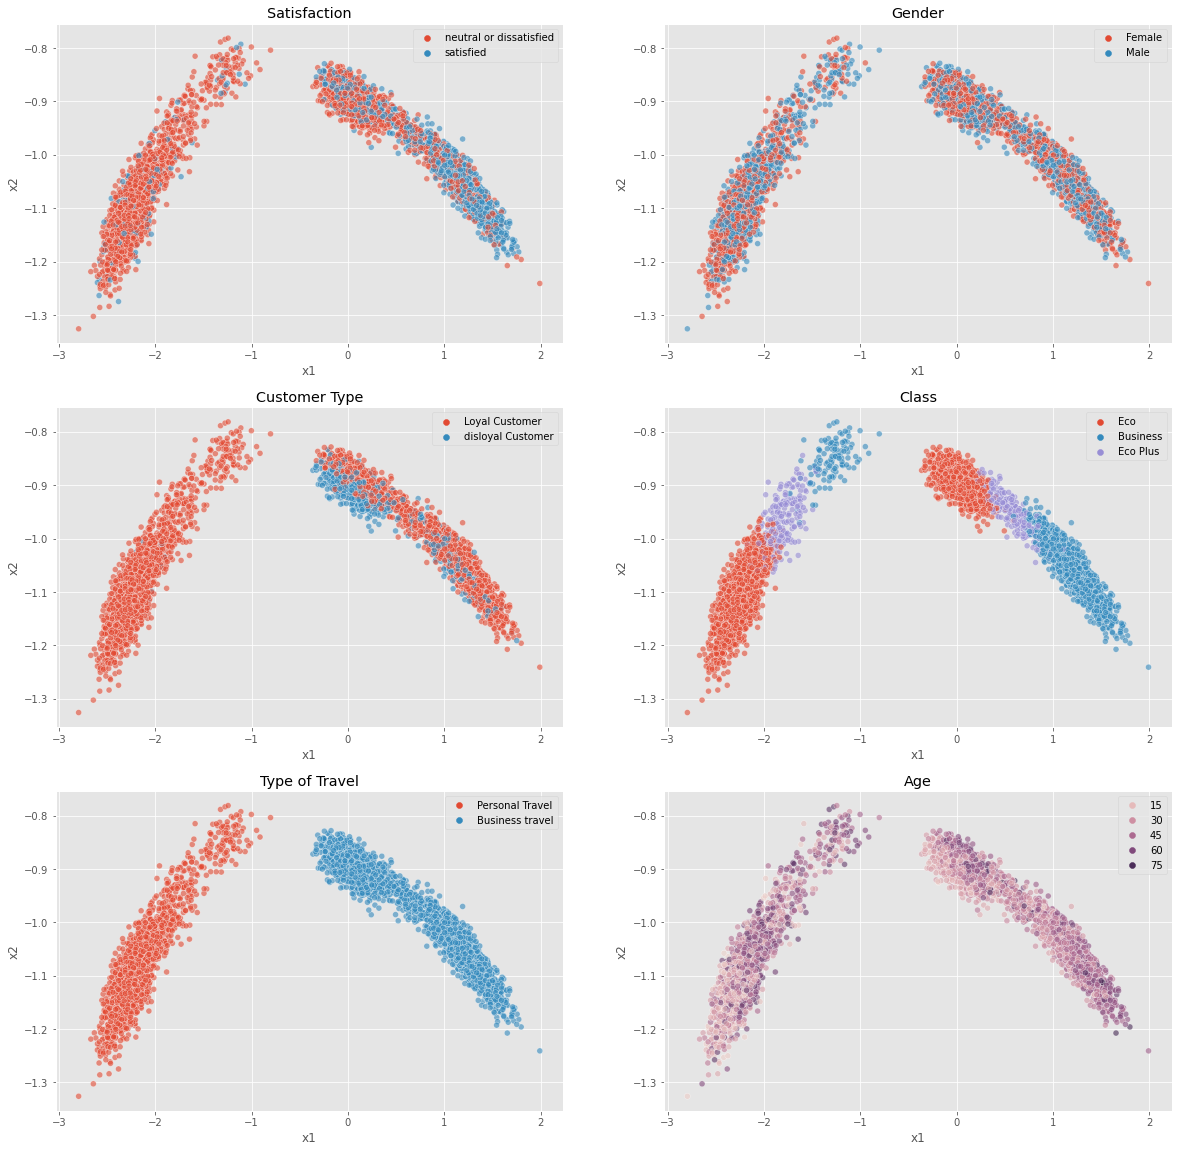
\includegraphics[width=0.7\textwidth]{node2vec_emb.png}
		\caption{Node2Vec embeddings}
        \label{fig:node2vec}
  \end{figure}

  \noindent The embeddings reveal very interesting insights in term of cluster
  analysis. First, the observation seen in figure \ref{fig:us_airline_graph}
  mainly correspond to the observations in figure \ref{fig:node2vec}. The
  advantage of graph representation learning, is that the nodes plotted using
  Node2Vec corresponds to a proper scatter plot in Euclidean space. In
  addition, the nodes are group in a much nicer and more orderly fashion. This
  makes it possible to infer with a higher level of certainty that for instance
  business class passengers traveling for business purposes tend to be more
  satisfied than other passengers on average. The 2 dimensional node embeddings
  thus provide interesting insights for cluster analysis. \\

  \noindent The node embeddings were used for three standard machine learning
  methods which are presented in table \ref{table:node2vec_results}.

  \begin{table}[h]
    \centering
    \begin{tabular}{|l||l|l|}
      \hline
      \textbf{ML Method} & \textbf{Training Accuracy} & \textbf{Validation
      Accuracy}\\
      \hline\hline
      Logistic Regression & 76.85\% & 75.83\% \\\hline 
      Support Vector Machine & 76.95\% & 75.66\% \\\hline
      ANN & 77.61\% & 76.58\% \\
      \hline
    \end{tabular}
    \caption{Node2Vec Classification Results}
    \label{table:node2vec_results}
  \end{table}

  \noindent The results show, that Node2Vec only has very modest success in
  classifying passengers according to their satisfaction. When looking at the
  satisfaction scatter plot in figure \ref{fig:node2vec} it becomes obvious why
  the downstream machine learning tasks only had limited success. For the
  variables which were used for generating the graph and for which neighborhood
  clusters emerged, Node2Vec created very good node embeddings. The label
  variable satisfaction could not be used for the graph generation as this would
  be unrealistic. Since the label is not considered for the graph generation,
  Node2Vec does not create embeddings which consider the label. The label is
  only considered to the extend that the variables used for the graph
  generation process create structures which are related somehow to the label.
  For that reason, the success of any downstream machine learning method will
  be limited to the extent that the node embeddings capture relevant information
  for predicting the label. The Python code for generating the node embeddings 
  and the subsequent machine learning methods can be found in appendix X. 

  \subsection{Graph Neural Networks}

  This subsection will present the results using graph neural networks. As
  mentioned in section 2, GCN by \cite{kipf2016semi} and
  GraphSage by \cite{hamilton2017inductive} will be used for classifying the
  satisfaction of the US airline passenger dataset. The model specifications 
  and results are presented in the following subsections.

  \subsubsection{Graph Convolutional Network}

  The GCN was designed using the exact forward propagation function
  previously outlined in equation \ref{eq:GCN_forward}.

  \begin{equation}
	  Z = f(X,A) = \text{softmax}\left(\hat A \;\text{ReLu}\left(\hat A X
	  W^{(0)}\right)W^{(1)}\right)
      \label{eq:GCN_forward_1}
  \end{equation}

  \noindent The node features $X$ correspond to the 21 selected explanatory 
  variables of the US airline passenger dataset as described in section 3. The
  node features were standardized due to large differences between the
  variables in terms of scale. In addition, standardizing yielded significant
  performance improvements. The hidden layer size for both convolutional layers
  was set to 128 and the output layer was set to size 2 for the binary
  classification. The training loss was calculated using cross-entropy loss and 
  the model parameters were updated using the Adam optimizer
  \citep{kingma2014adam} with the learning rate set to $0.01$. Essentially,
  algorithm \ref{algo:GNN_struct} ca be applied by replacing the forward
  propagation with equation \ref{eq:GCN_forward_1} and the model parameters are
  updated with the Adam optimizer instead of standard gradient descent.
  Different model specification were tested, however the chosen specifications
  appeared to perform very well. For example, choosing a hidden layer size of
  100 or 128 yielded virtually identical results. A stronger reduction in
  hidden layer size however reduces the performance of the GCN. Adding additional
  convolutional layers decreased the improvements and decreasing the learning
  rate decreased the performance. This graph convolutional network requires
  approximately 1'200 epochs to finish training. The loss- and accuracy plots
  are shown in figure \ref{fig:gcn_plots}.

  \begin{figure}[h]
		\centering
		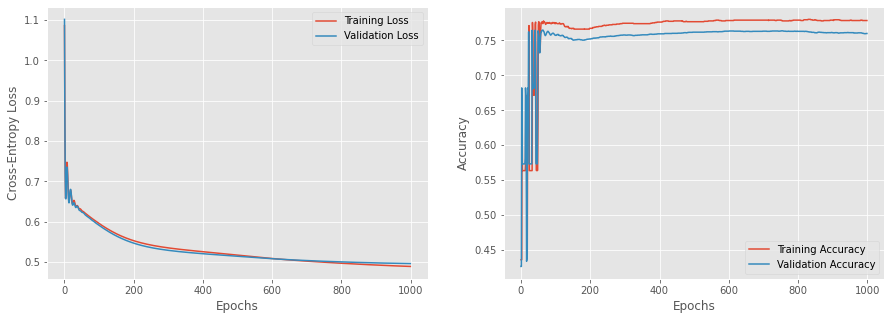
\includegraphics[width=0.7\textwidth]{gcn_plots.png}
		\caption{GCN Loss- and Accuracy Plots}
        \label{fig:gcn_plots}
  \end{figure}

  \noindent The results are are further presented in table
  \ref{table:gcn_results_train} \& \ref{table:gcn_results_valid}. 

  \begin{table}[h]
    \centering
    \begin{tabular}{|l|c|c|}
      \hline
      \diagbox{\textbf{Label}}{\textbf{Predicted}} & \textbf{Neutral or
      Dissatisfied} & \textbf{Satisfied}\\
      \hline
      \textbf{Neutral or Dissatisfied} & 893 & 143 \\\hline 
      \textbf{Satisfied} & 148 & 605 \\\hline\hline
      \textbf{Accuracy} & 83.73\% & \\
      \hline
    \end{tabular}
    \caption{Confusion Matrix Training Data}
    \label{table:gcn_results_train}
  \end{table}

  \begin{table}[h]
    \centering
    \begin{tabular}{|l|c|c|}
      \hline
      \diagbox{\textbf{Label}}{\textbf{Predicted}} & \textbf{Neutral or
      Dissatisfied} & \textbf{Satisfied}\\
      \hline
      \textbf{Neutral or Dissatisfied} & 2'004 & 383 \\\hline 
      \textbf{Satisfied} & 339 & 1'485 \\\hline\hline
      \textbf{Accuracy} & 82.85\% & \\
      \hline
    \end{tabular}
    \caption{Confusion Matrix Validation Data}
    \label{table:gcn_results_valid}
  \end{table}

  \noindent Graph convolutional networks are designed to be used in a
  transductive setting and the model cannot be applied to new and unseen
  graphs. In this setting 30\% of the dataset was used for training and 70\% of
  the data was used for validation. This is done by masking the nodes in the
  graph which are part of the validations dataset. The masked nodes are 
  considered in the in the neighborhood function $\mathcal{N}(v)$, they are 
  however not considered as target nodes. Therefore, masked nodes are not use
  for updating the model parameters. The fact, that GCNs cannot be used in an
  inductive setting is very limiting. Further, the GCN requires over 1'200
  epochs to start finish training and yields only mediocre results in terms of
  accuracy and model fit. A reason for this could be that only a full-batch
  implementation for GCN was introduced. In addition, GCNs always consider the
  entire neighborhood set. Sampling the neighborhood and mini-batch training 
  which is an important ingredient of GraphSage and is introduced as an
  improved and superior GNN method in the following subsection.

  \subsubsection{GraphSage}

  For GraphSage the exact same data input was used as for the GCN. The 
  GraphSage model included 2 convolutional layers where both have a hidden 
  layer size of 128 and the output layer is of size 2. The model is defined
  using an adaptation of algorithm \ref{algo:GraphSage} where the normalizing
  procedure in line  11 is skipped. This was done, as normalizing decreased the
  performance of the model. Similar as for the GCN, the training graph is
  split into 80\% training and 20\% validation using node masking. The loss is
  calculated using cross-entropy and the model parameters are updated using the
  Adam optimizer with the learning rate set to 0.001 and is an adaptation 
  to the model updating procedure shown in algorithm \ref{algo:GNN_struct}.
  The output of the first convolutional layer is activated using the ReLu 
  function and the output of the second convolutional layer is activated using 
  the softmax function. The model was trained using a mini-batch size of 50
  nodes and the neighborhood function $\mathcal{N}(v)$ randomly sampled 10
  neighbors for each node which are 2-hops away and randomly sampled 5 hidden 
  node representations which correspond to the activated output of the first 
  convolutional layer. This corresponds to the steps shown in figure
  \ref{fig:GraphSage_sample}. To improve the robustness of the model, lastly a
  dropout rate of 0.1 was set. GraphSage was run using the different
  aggregation strategies mean, LSTM and max-pooling. 
